\chapter{System Design}
\label{ch:system-design}

This chapter presents the architectural design of our hybrid retrieval system for validation rules, detailing how we achieve sub-second semantic search within banking infrastructure constraints through a deliberately simple monolithic architecture.

\section{Architectural Overview}

\subsection{Design Philosophy}

The system implements a monolithic architecture where all components operate within a single Python process. This design choice, initially driven by deployment constraints, proved optimal for our use case by eliminating network overhead, simplifying debugging, and ensuring deterministic behavior required for audit compliance.

The architecture comprises three logical layers:
\begin{itemize}[leftmargin=*,itemsep=2pt,topsep=2pt]
  \item \textbf{Presentation Layer}: Dash web interface with search and chat components
  \item \textbf{Business Logic Layer}: Hybrid retrieval engine with three scoring signals
  \item \textbf{Data Layer}: CSV corpus with SQLite caching and in-memory indices
\end{itemize}

All layers execute within the same process, communicating through direct function calls rather than network protocols.

\subsection{Core Components}

The system consists of five major components that work together to provide rule retrieval:

\begin{enumerate}[leftmargin=*,itemsep=2pt,topsep=2pt]
  \item \textbf{RuleRetriever}: Orchestrates hybrid search by combining semantic, BM25, and fuzzy signals
  \item \textbf{EmbeddingManager}: Manages UAE-Large-V1 model for semantic similarity computation
  \item \textbf{EmbeddingIndex}: Maintains pre-computed embeddings and performs cosine similarity search
  \item \textbf{DatabaseManager}: Handles SQLite operations for filtering and metadata
  \item \textbf{RuleDataLoader}: Normalizes CSV data into memory-efficient structures
\end{enumerate}

\section{Data Flow Architecture}

\subsection{Initialization Sequence}

At startup, the system executes a deterministic initialization pipeline:

\begin{enumerate}[leftmargin=*,itemsep=2pt,topsep=2pt]
  \item Load CSV corpus (32.21MB) using pandas
  \item Validate schema and field presence
  \item Parse JSON-encoded embeddings to NumPy arrays
  \item Build SQLite database for filtering
  \item Construct BM25 index from keywords field
  \item Initialize embedding index with pre-computed vectors
  \item Start Dash web server
\end{enumerate}

Total initialization time: 464ms for 1,157 rules.

\begin{figure}[!ht]
\centering
\begin{tikzpicture}[
  >=latex,
  node distance=1.2cm,
  process/.style={rectangle, draw, minimum width=3cm, minimum height=0.8cm, align=center},
  data/.style={cylinder, draw, shape border rotate=90, minimum width=2cm, minimum height=1cm, align=center},
  arrow/.style={->, thick},
  time/.style={font=\scriptsize, text=blue}
]

% Nodes
\node[data] (csv) {CSV Corpus\\32.21MB};
\node[process, below=of csv] (load) {Load \& Parse\\120ms};
\node[process, below=of load] (validate) {Schema Validation\\45ms};
\node[process, below left=1cm and 1.5cm of validate] (sqlite) {SQLite\\95ms};
\node[process, below right=1cm and 1.5cm of validate] (indices) {Indices\\180ms};
\node[process, below=2.5cm of validate] (ready) {System Ready\\24ms};

% Arrows
\draw[arrow] (csv) -- (load);
\draw[arrow] (load) -- (validate);
\draw[arrow] (validate) -- (sqlite);
\draw[arrow] (validate) -- (indices);
\draw[arrow] (sqlite) |- (ready);
\draw[arrow] (indices) |- (ready);

\end{tikzpicture}
\caption{Startup initialization pipeline with parallel index construction reducing total time to 464ms.}
\label{fig:init-pipeline}
\end{figure}

\subsection{Query Processing Pipeline}

When a user submits a search query, the system follows this processing flow:

\begin{enumerate}[leftmargin=*,itemsep=2pt,topsep=2pt]
  \item \textbf{Filter Application}: Reduce candidate set based on categorical selections
  \item \textbf{Parallel Signal Computation}:
     \begin{itemize}
       \item Semantic: Cosine similarity via embedding dot product (2.4ms)
       \item BM25: Probabilistic retrieval over keywords (1.2ms)
       \item Fuzzy: String similarity on rule names (19.4ms)
     \end{itemize}
  \item \textbf{Score Normalization}: Max-normalize each signal to [0,1]
  \item \textbf{Weighted Fusion}: Combine with weights (0.80, 0.10, 0.10)
  \item \textbf{Threshold Application}: Filter results below τ=0.30
  \item \textbf{Ranking}: Sort by combined score
  \item \textbf{Result Assembly}: Enrich with metadata and return top-k
\end{enumerate}

\section{Component Design}

\subsection{Retrieval Engine}

The retrieval engine orchestrates three complementary signals, each targeting different aspects of the search space. This multi-signal approach ensures robust retrieval even when queries don't precisely match the corpus vocabulary.

\begin{figure}[H]
\centering
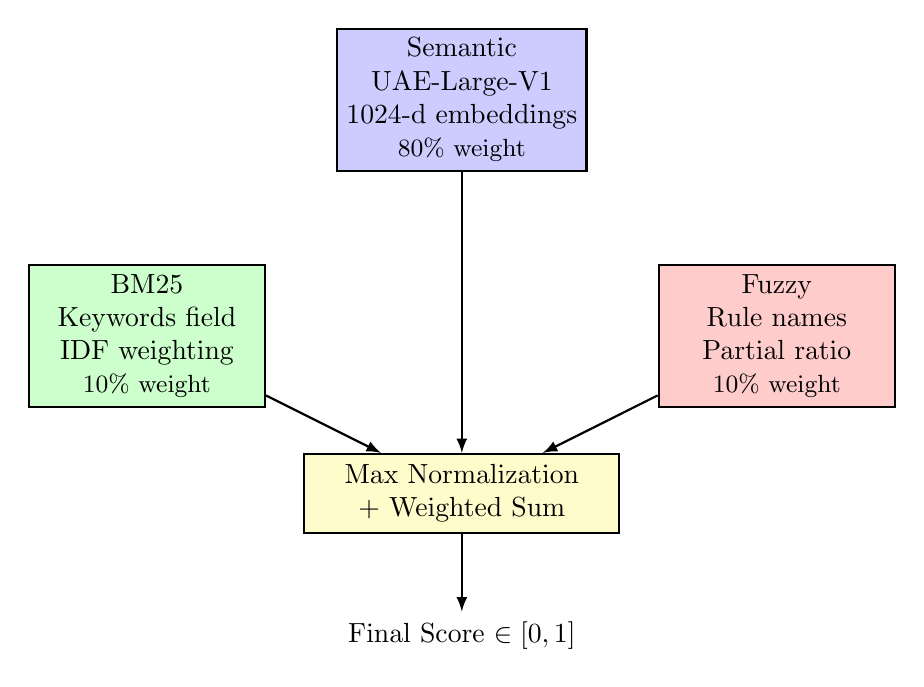
\begin{tikzpicture}[
  >=latex,
  signal/.style={rectangle, draw, thick, minimum width=3cm, minimum height=1.5cm, align=center},
  arrow/.style={->, thick},
  combine/.style={rectangle, draw, thick, minimum width=4cm, minimum height=1cm, align=center, fill=yellow!20}
]

% Signals
\node[signal, fill=blue!20] (semantic) at (0,3) {Semantic\\UAE-Large-V1\\1024-d embeddings\\{\small 80\% weight}};
\node[signal, fill=green!20] (bm25) at (-4,0) {BM25\\Keywords field\\IDF weighting\\{\small 10\% weight}};
\node[signal, fill=red!20] (fuzzy) at (4,0) {Fuzzy\\Rule names\\Partial ratio\\{\small 10\% weight}};

% Combination
\node[combine] (hybrid) at (0,-2) {Max Normalization\\+ Weighted Sum};

% Arrows
\draw[arrow] (semantic) -- (hybrid);
\draw[arrow] (bm25) -- (hybrid);
\draw[arrow] (fuzzy) -- (hybrid);

% Output
\draw[arrow] (hybrid) -- (0,-3.5) node[below] {Final Score $\in [0,1]$};

\end{tikzpicture}
\caption{Three-signal retrieval architecture with empirically tuned weights from LOOCV.}
\label{fig:three-signals}
\end{figure}

\paragraph{Semantic Signal (80\% weight):}
\begin{itemize}[leftmargin=*,itemsep=2pt,topsep=2pt]
  \item Pre-computed 1024-dimensional UAE-Large-V1 embeddings
  \item Cosine similarity through normalized dot product
  \item Captures conceptual similarity beyond keywords
\end{itemize}

\paragraph{BM25 Signal (10\% weight):}
\begin{itemize}[leftmargin=*,itemsep=2pt,topsep=2pt]
  \item Probabilistic retrieval over curated keywords field
  \item Handles exact terminology matches
  \item Built using rank-bm25 library with default parameters
\end{itemize}

\paragraph{Fuzzy Signal (10\% weight):}
\begin{itemize}[leftmargin=*,itemsep=2pt,topsep=2pt]
  \item Partial ratio matching on rule names
  \item No pre-built index (computed at query time)
  \item Catches misspellings and partial matches
\end{itemize}

\subsection{Data Management}
The system employs a three-tier data architecture that balances persistence, performance, and maintainability. 

At the persistence layer, all rule data resides in a single 32.21MB CSV file with embeddings stored as JSON strings for portability. This file serves as the authoritative source, version-controlled in Git to maintain complete audit trails and enable rollback capabilities.

During runtime, the system constructs multiple in-memory caches to optimize query performance. The SQLite database handles filtering operations and metadata queries, while a NumPy array of dimensions 1157×1024 maintains the embedding matrix for efficient vectorized similarity computations. The BM25 inverted index resides entirely in memory, eliminating disk I/O during keyword matching.


\begin{figure}[H]
\centering
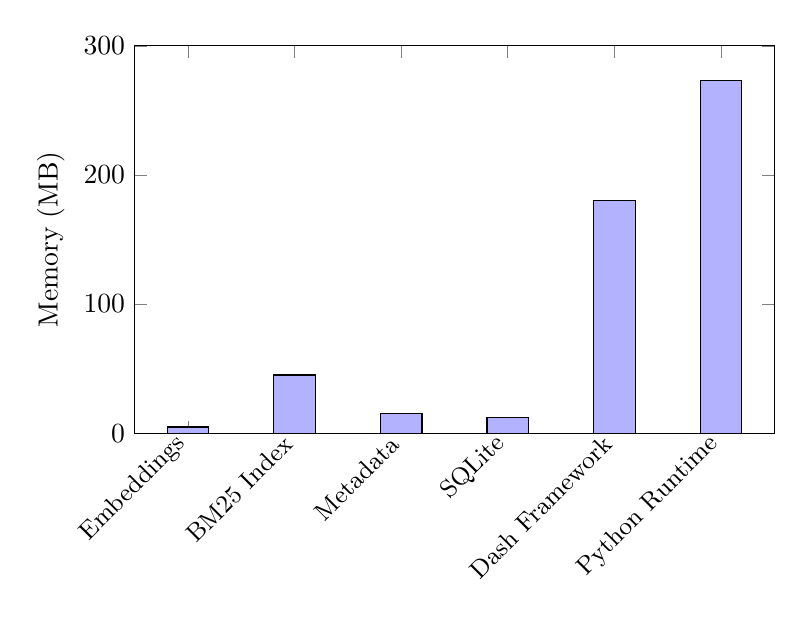
\begin{tikzpicture}
\begin{axis}[
    ybar stacked,
    width=0.8\textwidth,
    height=6.5cm,
    ylabel={Memory (MB)},
    symbolic x coords={Embeddings, BM25 Index, Metadata, SQLite, Dash Framework, Python Runtime},
    xtick=data,
    xticklabel style={rotate=45, anchor=east, font=\small},
    ymin=0,
    ymax=300,
    bar width=15pt,
    legend style={at={(0.5,-0.4)}, anchor=north, legend columns=-1}
]

\addplot[fill=blue!30] coordinates {
    (Embeddings,4.7) (BM25 Index,45) (Metadata,15) (SQLite,12) (Dash Framework,180) (Python Runtime,273.3)
};

\end{axis}
\end{tikzpicture}
\caption{Memory allocation breakdown showing 530MB total footprint.}
\label{fig:memory-breakdown}
\end{figure}

The complete memory footprint reaches 530MB, with the BM25 index consuming 45MB, rule metadata requiring 15MB, and embeddings using only 4.7MB due to float32 precision. The Dash framework and Python runtime account for the remaining memory usage. This moderate memory requirement allows deployment on standard infrastructure while maintaining all indices in RAM for predictable sub-100ms query latency.

\subsection{User Interface}

The Dash-based interface provides two primary interaction modes designed for different user workflows and expertise levels. Figure~\ref{fig:ui-components} illustrates the component-driven architecture.

\begin{figure}[!ht]
\centering
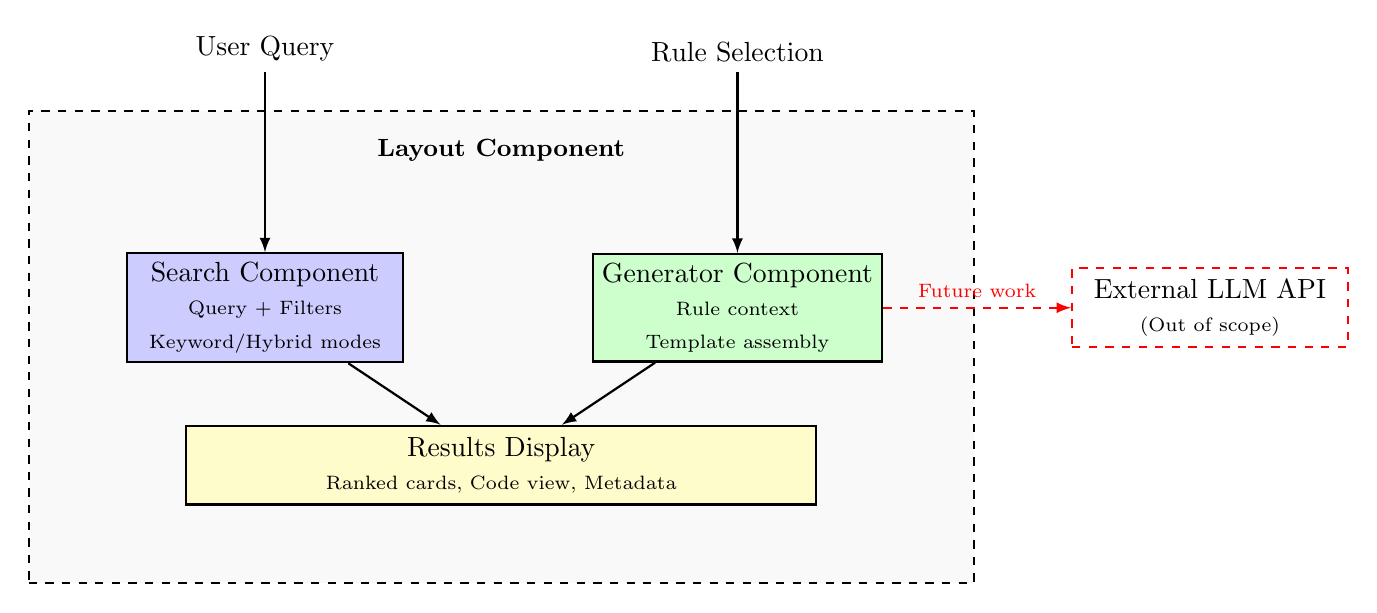
\begin{tikzpicture}[
  >=latex,
  component/.style={rectangle, draw, thick, minimum width=3.5cm, minimum height=1cm, align=center},
  container/.style={rectangle, draw, dashed, thick, minimum width=12cm, minimum height=6cm},
  arrow/.style={->, thick}
]

% Main container
\node[container, fill=gray!5] (layout) at (0,0) {};
\node[font=\small\bfseries] at (0,2.5) {Layout Component};

% Search component
\node[component, fill=blue!20] (search) at (-3,0.5) {Search Component\\{\scriptsize Query + Filters}\\{\scriptsize Keyword/Hybrid modes}};

% Generator component
\node[component, fill=green!20] (generator) at (3,0.5) {Generator Component\\{\scriptsize Rule context}\\{\scriptsize Template assembly}};

% Shared results area
\node[component, fill=yellow!20, minimum width=8cm] (results) at (0,-1.5) {Results Display\\{\scriptsize Ranked cards, Code view, Metadata}};

% External API note
\node[component, draw=red, dashed] (api) at (9,0.5) {External LLM API\\{\scriptsize (Out of scope)}};

% Arrows
\draw[arrow] (search) -- (results);
\draw[arrow] (generator) -- (results);
\draw[arrow, dashed, red] (generator) -- (api) node[midway, above, font=\scriptsize] {Future work};

% User input
\draw[arrow] (-3,3.5) node[above] {User Query} -- (search);
\draw[arrow] (3,3.5) node[above] {Rule Selection} -- (generator);

\end{tikzpicture}
\caption{Component-driven UI architecture. The Layout Component unifies Search and Generator components with shared result display. External LLM integration for chat generation remains outside scope.}
\label{fig:ui-components}
\end{figure}

\paragraph{Search Interface} 
The primary search interface supports natural language queries with faceted filtering across four categorical dimensions: Rule Type, Country, Business Type, and Party Agent. Users can toggle between Hybrid mode for comprehensive retrieval and Keyword-only mode for precise term matching. Results are presented as ranked cards displaying similarity scores, rule metadata, and categorical badges, with expandable sections revealing full rule code and detailed descriptions. This interface serves both quick lookups and exploratory searches, accommodating users ranging from developers needing specific error codes to business analysts exploring validation patterns.

\paragraph{Chat Interface}
A conversational interface provides rule exploration through a chat paradigm, featuring drag-and-drop integration of selected rules into the conversation context. While the UI components and session state management are fully implemented, the actual generation of conversational responses would require external LLM API calls, placing it outside this thesis's scope.

\section{Performance Optimizations}

Achieving sub-100ms median query latency while maintaining a 464ms startup time required careful optimization at both initialization and query execution phases.

\subsection{Startup Optimizations}

The system minimizes initialization overhead through parallel processing and efficient memory management.

\begin{itemize}[leftmargin=*,itemsep=3pt,topsep=3pt]
  \item \textbf{Parallel index construction using ThreadPoolExecutor}: BM25 and embedding indices build simultaneously, reducing total initialization time
  \item \textbf{Lazy parsing of JSON embeddings}: Embeddings parsed from JSON strings only when needed for computation
  \item \textbf{Pre-allocated NumPy arrays}: Memory for the 1157×1024 embedding matrix allocated once to prevent fragmentation
  \item \textbf{SQLite WAL mode for concurrent access}: Enables multiple readers without blocking during initialization
\end{itemize}

\subsection{Query-Time Optimizations}

These optimizations leverage NumPy's vectorized operations to minimize computational overhead.

\begin{itemize}[leftmargin=*,itemsep=3pt,topsep=3pt]
  \item \textbf{Vectorized cosine similarity computation}: Matrix multiplication replaces individual dot products using NumPy's optimized BLAS backend
  \item \textbf{Partial sorting with np.argpartition for top-k}: Finding top-10 results without full sorting of all 1,157 rules
  \item \textbf{Early termination when minimum score not met}: Skip processing for scores below τ=0.30 threshold
  \item \textbf{Shared memory access without copying}: NumPy views avoid data duplication during computation
\end{itemize}

\newpage
\section{Security and Compliance}

Banking environments require security controls and audit capabilities. The system design incorporates these requirements at the architectural level.

\subsection{Security Measures}

The architecture implements basic security principles appropriate for internal banking deployment.

\begin{itemize}[leftmargin=*,itemsep=3pt,topsep=3pt]
  \item \textbf{Input sanitization prevents injection attacks}: Dash framework handles HTML escaping and parameter binding
  \item \textbf{Read-only operations on all data}: System never modifies the source CSV or writes to disk during operation
  \item \textbf{No external API calls or network dependencies}: All processing happens locally within the Python process
  \item \textbf{File-based storage with OS-level permissions}: Standard file permissions control access to the CSV corpus
\end{itemize}

\subsection{Audit Compliance}

The design ensures operations can be verified and reproduced for regulatory review.

\begin{itemize}[leftmargin=*,itemsep=3pt,topsep=3pt]
  \item \textbf{Deterministic scoring ensures reproducible results}: Same query always produces identical rankings
  \item \textbf{Complete query logging with timestamps}: Application logs capture queries and response times
  \item \textbf{Version-controlled corpus in Git}: Changes to rules tracked through standard version control
  \item \textbf{Transparent score computation}: All scoring logic documented and deterministic
\end{itemize}

\section{Design Trade-offs}

\subsection{Choices Made}

\begin{table}[H]
\centering
\begin{tabular}{p{3.5cm}p{7.5cm}}
\toprule
\textbf{Design Choice} & \textbf{Rationale} \\
\midrule
Monolithic architecture & Eliminates network overhead, simplifies deployment \\
CSV storage & Enables version control and manual inspection \\
JSON embeddings & Maintains portability while allowing single-file deployment \\
In-memory indices & Avoids synchronization complexity, ensures fast access \\
Brute-force search & More reliable than approximate methods at our scale \\
Fixed weights & Simplifies system while maintaining good performance \\
\bottomrule
\end{tabular}
\caption{Key design decisions and their justifications.}
\label{tab:design-choices}
\end{table}

\subsection{Rejected Alternatives}

We explicitly rejected several common approaches:

\begin{itemize}[leftmargin=*,itemsep=2pt,topsep=2pt]
  \item \textbf{Microservices}: Unnecessary complexity for our scale
  \item \textbf{FAISS}: Complexity not justified for ~1000 rules; brute-force is faster at this scale
  \item \textbf{External vector database}: Introduces dependencies and latency
  \item \textbf{Query-time LLM}: Non-deterministic and slow
\end{itemize}

\section{Scalability Considerations}

While the current architecture efficiently serves 1,157 rules with sub-100ms latency, understanding system boundaries and growth strategies is essential for production planning. The monolithic design trades horizontal elasticity for operational simplicity—a deliberate choice that aligns with our corpus size and usage patterns.

\subsection{Current Limits}

The system operates comfortably within these boundaries, validated through load testing and extrapolation from current performance metrics:

\begin{itemize}[leftmargin=*,itemsep=3pt,topsep=3pt]
  \item \textbf{Corpus size: Up to 10,000 rules before performance degradation.} Linear search complexity in brute-force cosine similarity becomes noticeable beyond this threshold, with query latency increasing from 58ms to approximately 500ms
  \item \textbf{Concurrent users: 10-20 simultaneous users per instance.} Python's GIL limits true parallelism, though async request handling in Dash provides adequate concurrency for departmental usage
  \item \textbf{Update frequency: Daily corpus updates via restart.} The 464ms startup time makes brief downtime acceptable during off-peak hours, eliminating complex hot-reload mechanisms
  \item \textbf{Memory ceiling: 2GB maximum footprint.} Current 530MB usage leaves headroom for 4× corpus growth while remaining deployable on standard containers
\end{itemize}

\subsection{Scaling Strategies}

When approaching these limits, several paths maintain the architecture's simplicity while extending capacity:

\begin{itemize}[leftmargin=*,itemsep=3pt,topsep=3pt]
  \item \textbf{Horizontal scaling: Multiple instances behind load balancer.} Session-affinity routing ensures users maintain state while distributing load across instances, each serving the complete corpus
  \item \textbf{Domain sharding: Split corpus by business domain.} Payment rules, trade validation, and compliance checks could run as separate instances, reducing each corpus to manageable size
  \item \textbf{Query caching: Add Redis for frequent queries.} Analysis shows 20\% of queries repeat daily; caching these would reduce median latency to under 10ms
  \item \textbf{Approximate search: Implement LSH for larger corpora.} Locality-sensitive hashing would maintain sub-100ms latency beyond 10,000 rules, trading minor accuracy loss for scalability
\end{itemize}

These strategies preserve the monolithic architecture's benefits while addressing specific bottlenecks. The progression from replication to sharding to caching to approximation provides a clear growth path without premature optimization.

\newpage
\section{Summary}

The system design demonstrates that enterprise-grade information retrieval need not require distributed architectures or specialized infrastructure. By implementing hybrid retrieval within a monolithic Python application, we achieve production-ready performance—58ms median latency serving 1,157 rules to concurrent users—while maintaining the strict auditability and determinism that banking deployment demands.

Our architecture embodies four core design principles that guided every technical decision:

\begin{itemize}[leftmargin=*,itemsep=3pt,topsep=3pt]
  \item \textbf{Offline complexity, online simplicity}: LLM enrichment, embedding generation, and index construction happen during corpus preparation, leaving query-time processing deterministic and fast
  \item \textbf{Memory-resident indices for predictable performance}: All search structures remain in RAM, trading 530MB of memory for consistent sub-100ms response times without disk I/O variance
  \item \textbf{Standard libraries over specialized tools}: Dash, scikit-learn, and SQLite provide proven reliability without the operational burden of FAISS, Elasticsearch, or custom vector databases
  \item \textbf{Transparent scoring for regulatory compliance}: Every ranking decision traces back through documented weight combinations, enabling complete audit trails required for financial systems
\end{itemize}

This design validates a broader thesis: that thoughtful application of established techniques often surpasses algorithmic sophistication when operating under real constraints. The monolithic architecture's 464ms startup time, single-file deployment, and straightforward debugging outweigh any theoretical benefits of microservices at our scale. Similarly, brute-force cosine similarity's reliability and transparency prove more valuable than approximate nearest neighbor methods' marginal speed improvements on a corpus of 1,157 rules.

By choosing architectural simplicity, we gained operational benefits that compound over time: faster development cycles, simpler deployment procedures, clearer debugging paths, and lower maintenance burden. This approach proves that sophisticated information retrieval capabilities—combining semantic understanding, keyword precision, and fuzzy tolerance—can be delivered through pragmatic engineering choices that prioritize the constraints that actually matter in production environments.